\section{Overview}
Pookie operates by analyzing video and audio inputs to assess the user's facial and speech emotions. It employs convolutional neural networks for facial emotion recognition and bidirectional LSTMs for speech emotion analysis. Based on the detected emotions, Pookie selects the most suitable interaction to engage with the user. For example, if the user appears sad, the robot may respond with a gentle sound, a cheerful expression, and slow, comforting movements to create a sense of empathy. This section will outline Pookie’s progress in semester 2, covering completed tasks, ongoing work, and future steps.
\subsection{What’s done}
Overall, the team has finalized the overarching approach of the interaction with the robot. This process was not well defined in the last semester, which led to ambiguity towards the final presentation. To elaborate, it was not clear of what output the robot would elicit given a certain combination of emotions. If the user was sad, should the robot try to cheer the user up? Or should it maintain neutrality. As such, the team has decided to consult Chula Student Wellness again for a quick chat to obtain their thoughts on this problem. They told us that the factors going into determining the output were almost infinite, where even psychologists themselves have problems truly empathizing with a person, and determining what to do to make a person feel better. As such, they claim it is almost impossible for our project to empathize to that extent. Therefore, we settled on a more generalized approach, as shown in Figure \ref{fig:flow}.

\begin{figure}[ht]
    \centering
    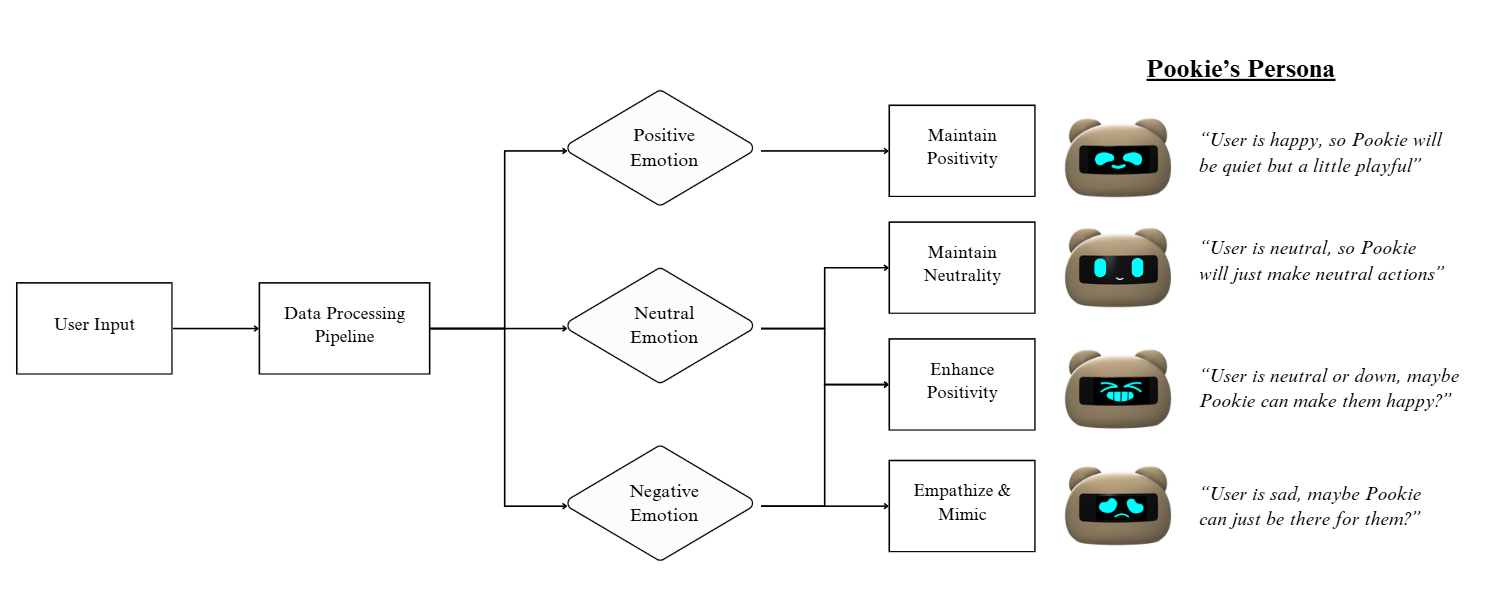
\includegraphics[width=\textwidth]{flow.png}
    \caption{Pookie Interaction Flowchart}
    \label{fig:flow}
\end{figure}

After processing inputs in the form of facial and speech emotion, the robot segments the output into 3 possible cases: positive, neutral and negative. With each case, the robot has a set of outputs it can perform. For instance, if the person is in a positive wellness state, Pookie will maintain positivity, meaning its intention will be to ensure this positive state of being of the user will be prolonged. On the other hand, if the user is neutral, Pookie will try to maintain this neutrality, but in some cases, such as if our models detect that the user is 60\% neutral, but 40\% happy, then the robot will elicit an output that could potentially make the user happier. Lastly, for the case of negative emotion, this part is tricky. The team has a design problem here: if the user is feeling negative, should the robot remain neutral? Should it show empathy? Or should it be fun and energetic? The underlying emotional factors, as we mentioned, are almost infinite, so we simplified it into two cases: either enhance positivity or empathize. In the case of empathy, the robot will simply mimic the user’s emotion (e.g sadness), with the intention of “being there” for the user. 

Another fundamental update is how Pookie processes the emotional inputs. Initially, the team finalized on the approach of finding the dominant emotion from the facial and speech emotion recognition models within a given time frame, then simply using those two dominant emotions to elicit an input. For instance, within 10 seconds, if a user made a “happy” face, and their speech is “happy”, then the output would be a positive maintenance. However, this approach disregarded many cases and made the robot very static. If the user’s face is “sad”, but their voice is “happy”, it’s impossible to combine these emotions and determine what the user’s true emotion is. This leads us to incorporating two new key technologies: bayesian networks and decision trees, creating a new flowchart as seen in Figure \ref{fig:rev_flow}.

\begin{figure}[ht]
    \centering
    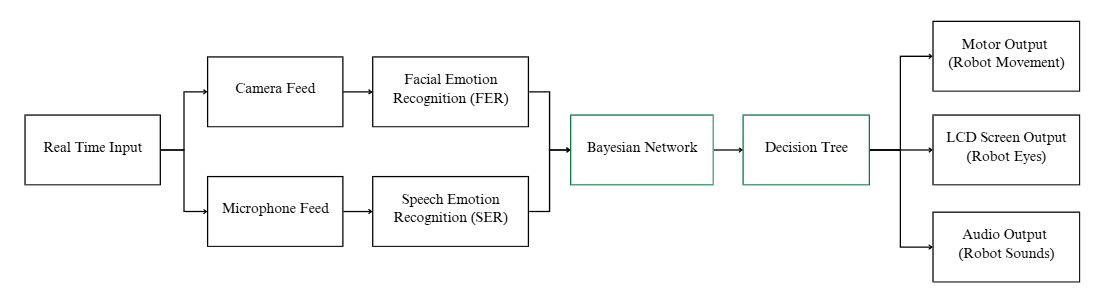
\includegraphics[width=\textwidth]{flow_revised.png}
    \caption{Revised Flowchart for Input Processing}
    \label{fig:rev_flow}
\end{figure}

The next update involves the implementation of the robot’s eyes, which is a fundamental interaction done through the LCD screen of the robot. Initially, the eyes of the robot used a Python library called OpenCV, which is an image processing library allowing the drawing of various shapes. The eyes were hard coded as various shapes and patterns drawn on a black canvas, as shown in Figure 3. The main challenge with this approach was the scalability and implementation time. Since each frame is hard coded, it does not allow for much flexibility and complex shapes. However, the upside is that it can easily be built in as a class into the main code. 

\begin{figure}[ht]
    \centering
    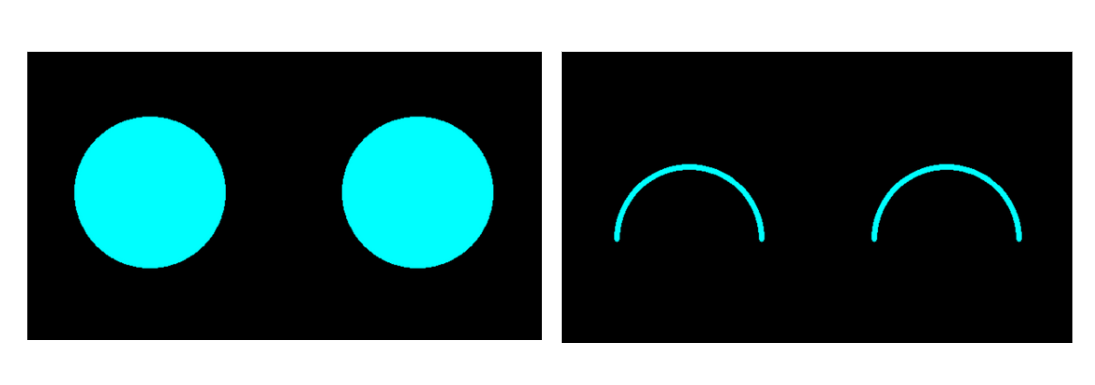
\includegraphics[width=\textwidth]{happy.png}
    \caption{OpenCV Eyes Example for “Happy”}
    \label{fig:happy}
\end{figure}

The team decided on a different approach: using a simple software that could easily create dynamic shapes and record the frame sequence as a common file type, like GIF. The solution was Canva, a program typically used to make powerpoint slides, but with animation capabilities as well. Through implementing the eye sequence as a GIF format instead of hard coding, we are able to achieve more unique and personalized eye shapes and sequences for Pookie. Some examples of these are shown in Figure \ref{fig:new_eyes}.

\begin{figure}[ht]
    \centering
    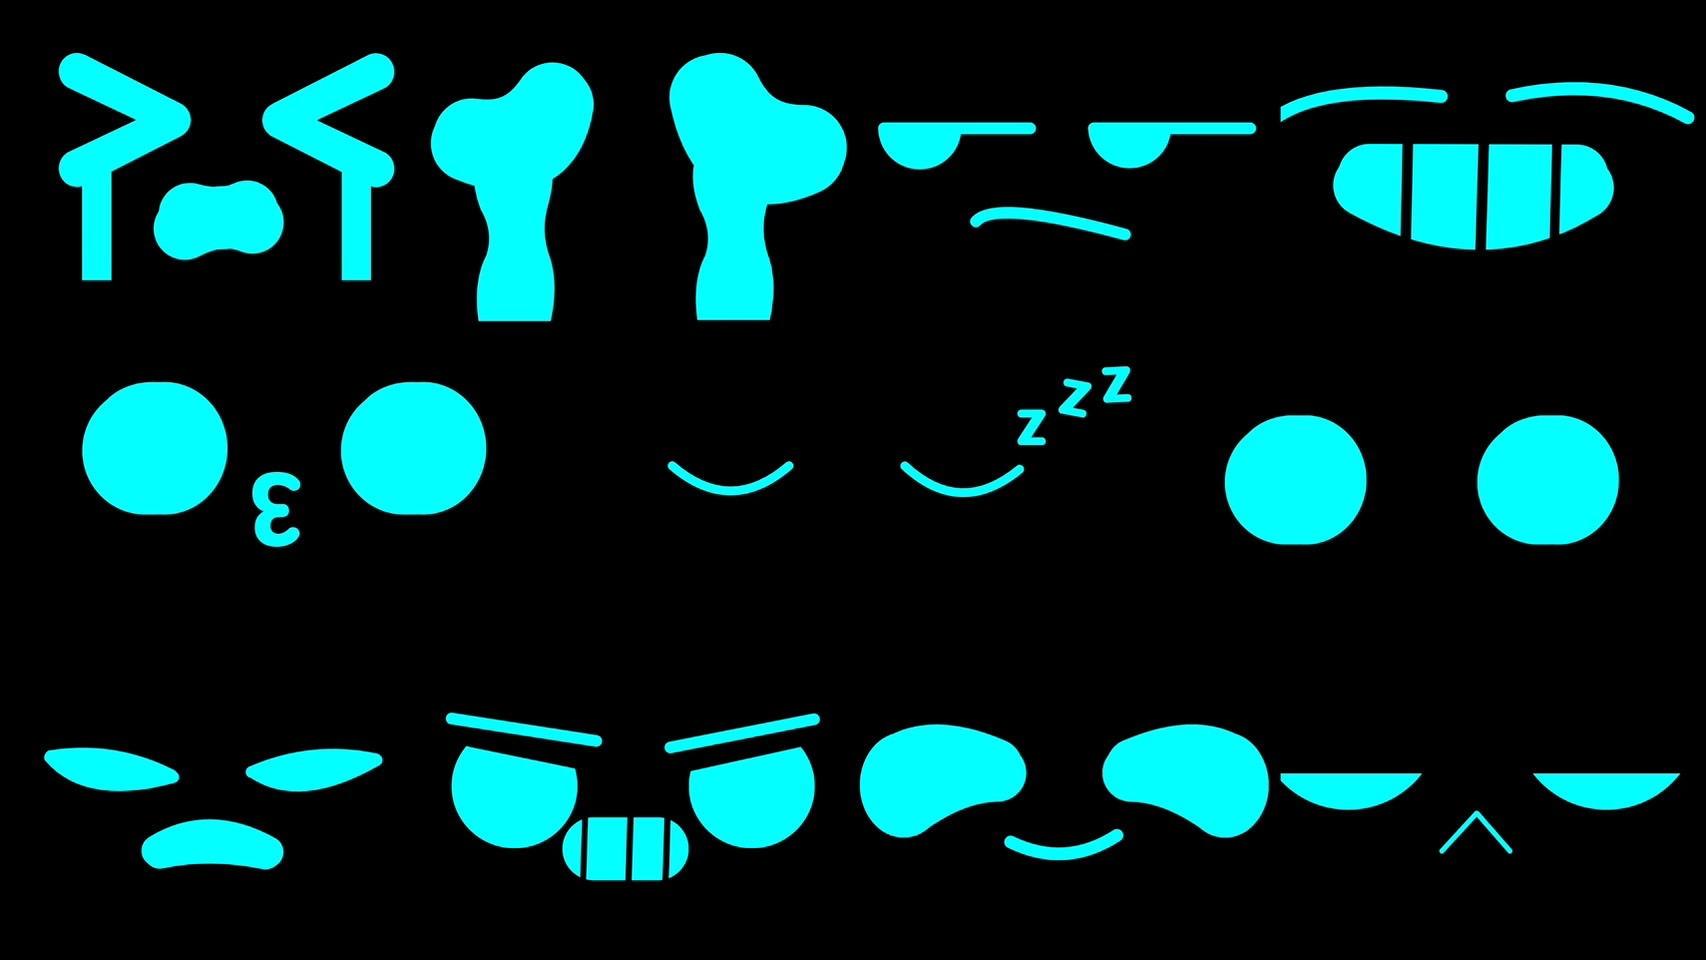
\includegraphics[width=\textwidth]{new_eyes.png}
    \caption{New Eyes Drawn as GIF Sequence on Canva}
    \label{fig:new_eyes}
\end{figure}

\newpage
Lastly, some other updates regard the hardware components. Our hardware team has completed a final design of Pookie in Fusion 360, and has acquired almost all necessary components needed for assembly. This will be discussed further in the hardware section.

\subsection{What we are working on}
This section discusses the currently ongoing tasks the team is working on this week and next week. Currently, the team is working on the Jetson Nano integration, which is the main processor for the project. Initially, in the last semester, the code, sensors, models, and so on were all hosted on a local computer, so it must be migrated and tuned so that it works appropriately with the Jetson Nano. Aside from this, we are working on coding the hardware functions, such as driving the servo motors, which are used to drive the arms, base, and neck of the robot. 

On the software side, although we have completed the Bayesian network, which is essential for predicting the user’s true emotion, the next part is also challenging: the decision tree. This requires the team to carefully design and process inputs. For instance, if the user is detected to be 50\% happy and 50\% sad at the same time, what does this constitute? Which set of actions should the robot perform: positive enhancement or maintenance. The team is working on carefully building this tree everyday, a few nodes at a time.

